\documentclass[12pt] {report}
\usepackage{apacite}
\usepackage[spanish]{babel}
\usepackage{natbib}
\usepackage{url}
\usepackage[utf8x]{inputenc}
\usepackage{amsmath}
\usepackage{graphicx}
\graphicspath{{images/}}
\usepackage{parskip}
\usepackage{fancyhdr}
\usepackage{float}
\usepackage{vmargin}
\setmarginsrb{3 cm}{2.5 cm}{3 cm}{2.5 cm}{1 cm}{1.5 cm}{1 cm}{1.5 cm}

\title{Resultados de Investigación}				
\author{Br. Amayrani Soto Paul}		

\date{\today}								

\makeatletter
\let\thetitle\@title
\let\theauthor\@author 
\let\thedate\@date
\makeatother

\pagestyle{fancy}
\fancyhf{}
\rhead{\theauthor}
\lhead{\thetitle}
\cfoot{\thepage}
\begin{document}

%%%%%%%%%%%%%%%%%%%%%%%%%%%%%%%%%%%%%%%%%%%%%%%%%%%%%%%%%%%%%%%%%%%%%%%%%%%%%%%%%%%%%%%%%

\begin{titlepage}
	\centering
    \vspace*{0.2 cm}
    
\includegraphics[scale = 0.60]{log1.png}\\[3.0 cm]
          \textsc{\LARGE Instituto Tecnologico Superior de Escarcega}\\[2.0 cm]	% University Name
	\textsc{\Large EVALUACIÓN SOBRE SI LOS CONOCIMIENTOS EN LA RESOLUCIÓN DE ECUACIONES LINEALES INFLUYEN EN LAS HABILIDADES DE PROGRAMACIÓN. }\\[0.5 cm]				
	\textsc{\large Taller de Investigación II}\\[0.5 cm]				
	\rule{\linewidth}{0.2 mm} \\[0.4 cm]
	{ \huge \bfseries \thetitle}\\
    
	\rule{\linewidth}{0.2 mm} \\[1.5 cm]
	
	\begin{minipage}{0.4\textwidth}
		\begin{flushleft} \large
			\emph{Elaboró:}\\
			\theauthor
			\end{flushleft}
			\end{minipage}~
			\begin{minipage}{0.4\textwidth}
			\begin{flushright} \large
			\emph{Asesor:} \\
			Ing. Manuel Arturo Suarez Amendola,MC	
           
		\end{flushright}
        
	\end{minipage}\\[2 cm]
	
	{\large \thedate}\\[5 cm]
 
	\vfill
	
\end{titlepage}

%%%%%%%%%%%%%%%%%%%%%%%%%%%%%%%%%%%%%%%%%%%%%%%%%%%%%%%%%%%%%%%%%%%%%%%%%%%%%%%%%%%%%%%%%

\tableofcontents
\pagebreak

%%%%%%%%%%%%%%%%%%%%%%%%%%%%%%%%%%%%%%%%%%%%%%%%%%%%%%%%%%%%%%%%%%%%%%%%%%%%%%%%%%%%%%%%%

\section{Resumen}
El presente proyecto trata sobre la relación que existe entre las habilidades con las que cuenta un estudiante de ingeniería en la resolución de ecuaciones y las de programación.\\
La comprobación de la hipótesis se realizó mediante la aplicación de una encuesta para identificar los hábitos de estudio de cada alumno y dos exámenes para medir el nivel académico con el que cuentan los exámenes fueron de programación y resoluciones de ecuaciones.\\
El impacto que tiene la realización de este proyecto, a grandes rasgos es ubicar con qué nivel académico cuentan los estudiantes pertenecientes a la carrera de ingeniería en sistemas computacionales y determinar en qué aspectos deberían de mejorar los profesores para que un alumno sea capaz de generar una solución a diversos problemas por medio de un lenguaje de programación y además identificar si realmente las habilidades matemáticas, influyen directamente en el aprendizaje y razonamiento de los estudiantes para generar soluciones a dichos problemas.\\

\section{Abstract}

This project deals with the relationship between the abilities of an engineering student in solving equations and those of programming.\\
The test of the hypothesis was carried out by means of the application of a survey to identify the habits of study of each student and two exams to measure the academic level with which they counted the examinations were of programming and resolutions of equations.\\
The impact of this project, in broad strokes is to locate with what academic level the students belonging to the engineering career in computational systems count and determine in which aspects they should improve the teachers so that a student is able to generate a Solution to various problems through a programming language and also identify if mathematical skills really directly influence students' learning and reasoning to generate solutions to such problems.\\
\\

\textbf{\small Keywords: face detectors, safety systems, impact, benefit, feasibility, hypothesis}.

\section{Introducción}
Identificar las habilidades de programación en los alumnos es un tema muy importante, debido a que la mayoría de los alumnos pertenecientes a la carrera de ingeniería en sistemas computacionales carece de conocimientos en esa área, lo cual representa un problema bastante alarmante porque estos conocimientos son indispensables para el perfil de un ingeniero.\\
Por ello en este proyecto, el tema a tratar es un poco complejo, debido a que fue un poco tedioso elegir los factores que influyen directamente para que un alumno carezca de habilidades en el área de programación, ya que esta situación se puede deber a diversas circunstancias pero para obtener resultados más concretos solo se tomaran en cuenta una de esas causas.\\ 
En la presente investigación se compara la relación que existe entre las habilidades matemáticas y de programación, por ejemplo un alumno que cursa alguna de esas asignaturas puede tener mayor desempeño en alguna de ellas y estar bajo en la otra.\\
La programación es una habilidad muy útil para un profesionista y su práctica puede ser muy gratificante. En los últimos años la demanda de programadores se ha incrementado, y por supuesto también el interés de los jóvenes por cursar carreras relacionadas con la programación. Del mismo modo, los cursos introductorios de programación se han vuelto cada vez más populares en las diversas carreras universitarias.\\
Sin embargo, aprender a programar no parecer tarea fácil. Muchos programadores principiantes se enfrentan a una amplia gama de dificultades y deficiencias, lo que ha causado que se considere a los cursos de programación como una labor difícil. Lo anterior no es fácil negar si consideramos que estos cursos con frecuencia son los que muestran las tasas más altas de deserción escolar y de reprobación. 
Por esta y diversas razones en este proyecto se estudia, a que se debe que un alumno tenga un desempeño bajo en programación, todo esto se lleva a cabo mediante una serie de pruebas en las que se evalúa el nivel académico obtenido por los alumnos en las asignaturas relacionadas con la resolución de ecuaciones y generar soluciones a problemas por medio de programación en los semestres cursados en la carrera.\\
Con la comprobación de la hipótesis que se plantea en el transcurso de la investigación, se estará obteniendo alguno de los factores en que los alumnos deberían poner mayor atención y además de que a partir de la información obtenida se podrán generar soluciones a este problema, ya sea con la impartición de cursos para reforzar los conocimientos de los estudiante.\\ 
\\
\section{Tema de investigación}
Evaluación sobre si los conocimientos en la resolución de ecuaciones lineales influyen en las habilidades de programación.\\ 
\section{Pregunta de investigación}
¿Es la falta de conocimientos en la resolución de ecuaciones lineales un factor importante para el desarrollo de las habilidades en la elaboración de software matemático? \\ 
\\ 
 


\section{Marco teórico}
En (Edgar Javier Moreno, 1903) diversos autores realizan una investigación, la cual expone las características y virtudes del trabajo colaborativo, el cual puede abordarse como una metodología apropiada para enriquecer el proceso enseñanza-aprendizaje.\\ 
El objetivo de este trabajo es proponer mecanismos para implementar la metodología en los primeros niveles de programación en el ámbito universitario. 
Actualmente hay una fuerte tendencia a utilizar distintas herramientas en la nube (sobre internet) las cuales pueden contribuir a facilitar el trabajo colaborativo. Se mencionarán herramientas de acceso fácil para los alumnos en su mayoría “nativos tecnológicos” y posteriormente se realizará un análisis de otros software no tan difundidos desarrollados específicamente para implementar el trabajo colaborativo.\\ 
De acuerdo con esta información si se han realizado investigaciones acerca del tema y a pesar de que no tengan el mismo enfoque  contribuyen en gran medida al desarrollo de este proyecto, debido a que nos habla un poco sobre la mejorar el proceso de aprendizaje de los alumnos universitarios en el área de programación.\\
Por otro lado (Xabier Basogain Olabe, 2015) un grupo de profesores realizaron una investigación sobre el concepto del Pensamiento Computacional y cómo puede ser integrado en el aula a través del diseño e implementación de proyectos de programación. Se describe la necesidad, el propósito y las principales características del Pensamiento Computacional. Se muestra con varios ejemplos cómo se pueden desarrollar los elementos fundamentales del Pensamiento Computacional utilizando un lenguaje programación.\\
Dentro de su artículo se define el concepto de pensamiento computacional, el cual es una metodología basada en la implementación de los conceptos básicos de las ciencias de la computación para resolver problemas cotidianos, diseñar sistemas domésticos y realizar tareas rutinarias.   
Toda esta información contribuye bastante a nuestra investigación ya que, nos muestra cómo debemos abordar un problema para luego traducirlo a algún leguaje de programación, de esta manera podemos transmitir este conocimiento a los alumnos que nos servirán de muestra para realizar nuestras pruebas en el transcurso de este proyecto.\\
Otra parte muy importante que vale la pena analizar son las competencias obtenidas al final de un curso por un alumno, por ello se decidió analizar (Marcha, 2010) ahí se presentan los estilos y evaluación del aprendizaje en la universidad, además de cómo identificar si un alumno obtuvo las competencias planeadas durante el curso.\\    
Después de comparar la información consultada en las distintas fuentes, se identificaron conceptos muy importantes para nuestro tema, como es la implementación del trabajo colaborativo al momento de resolver un problema a través de un lenguaje de programación.\\
También se habla sobre el pensamiento computacional, el cual es un concepto clave debido a que a veces el alumno puede resolver un  problema matemático de manera física pero no tiene el conocimiento o habilidades para poder implementarlo dentro de un programa con los mismos requerimientos.
Por ultimo están las competencias obtenidas por el alumno, es decir que al final de cada curso se deben de adquirir ciertos conocimientos y habilidades por parte del educando, por ello para el desarrollo de esta investigación se analizaran los documentos donde se encuentran plasmadas las competencias que se deben obtener tanto en la asignatura enfocada a programación como la de matemáticas para poder medir el desempeño de los alumnos.\\

  
\section{Hipótesis }
La falta de conocimiento en la resolución de ecuaciones lineales, si es considerado un factor importante para que el alumno cuente con habilidades para desarrollar un software matemático.\\
\section{Planteamiento del problema}
La idea surge con la identificación de un problema en la carrera de ingeniería en sistemas computacionales, el cual consiste en que un gran número de alumnos carece de conocimientos en el área de programación y probablemente este problema esté relacionado con las habilidades matemáticas.\\
Para el desarrollo de este proyecto se plantean una serie de objetivos para poder obtener resultados satisfactorios, estos se mencionan a continuación:\\
Ubicar a la población a la que se le aplicarán los instrumentos de evaluación.\\
Aplicar instrumentos de evaluación.\\
Generar gráficas de los resultados de los instrumentos de evaluación.\\
Interpretar la información obtenida.\\
A grandes rasgos estos son algunos de los objetivos a cumplir, pero cabe mencionar que la realización de esta investigación estará compuesta por un mayor número de actividades.\\
El que un alumno no pueda desarrollar sus habilidades en programación al 100 por ciento, no solo se debe, a que no cuente con conocimientos en matemáticas, también se puede deber a sus hábitos de estudio o a los profesores que le imparten la asignatura pero para el desarrollo de este proyecto solo tendremos en cuenta la relación entre la resolución de ecuaciones y encontrar soluciones a diversos problemas por medio de algún lenguaje de programación.\\
Esta investigación es importante, debido a que durante varias generaciones se ha identificado un bajo desempeño por parte de los alumnos en las asignaturas que emplean algún lenguaje de programación, por ejemplo de un grupo de hasta 25 estudiantes se podría decir que solo 5 por ciento domina por completo esta habilidad.\\
En cuanto al impacto que tendría la realización de este proyecto, a grandes rasgos seria ubicar con qué nivel académico cuentan los estudiante pertenecientes a la carrera y determinar en qué aspectos deberían de mejorar los profesores para que un alumno sea capaz de generar una solución a diversos problemas por medio de un lenguaje de programación y además identificar si realmente las habilidades matemáticas, influyen directamente en el aprendizaje y razonamiento de los estudiantes para generar soluciones a dichos problemas.\\
La importancia de que un alumno cuente con las habilidades necesarias en esta área radica en el hecho de que al momento de desempeñarse en el entorno laboral pueda obtener mayores oportunidades. \\ 
Como se mencionó al principio en la introducción hoy en día existe una gran competencia en la parte de desarrollo de software, debido a que la mayoría de las personas ya se interesa por aprender algún lenguaje de programación, en cierta manera es algo lamentable que un alumno no cuente con la habilidad de generar soluciones a problemas por medio de alguno de estos lenguajes, con el desarrollo de este proyecto estaríamos atacando alguno de los factores que influyen a que esto sea posible. \\
Para cumplir con los objetivos de la investigación y generar resultados que nos puedan orientar a la confirmación o rechazo de la hipótesis que se planteará, se tiene planeado aplicar encuestas y exámenes a los estudiantes para que a partir de la interpretación de la información obtenida se pueda obtener una posible solución a este problema.\\ 

\section{Resultados}
A continuación se presentan las gráficas de los resultados obtenidos con la aplicación de los instrumentos de evaluación.
\section{Gráficas de distribución de probabilidad }
\begin{figure}[H]
\centering
En la siguiente tabla se muestran los resultados obtenidos y con ello se obtiene información sobre si un alumno cuenta con un horario establecido para las asignturas relacionadas con matemáticas o simplemente realiza sus actividades en cual tiempo libre 
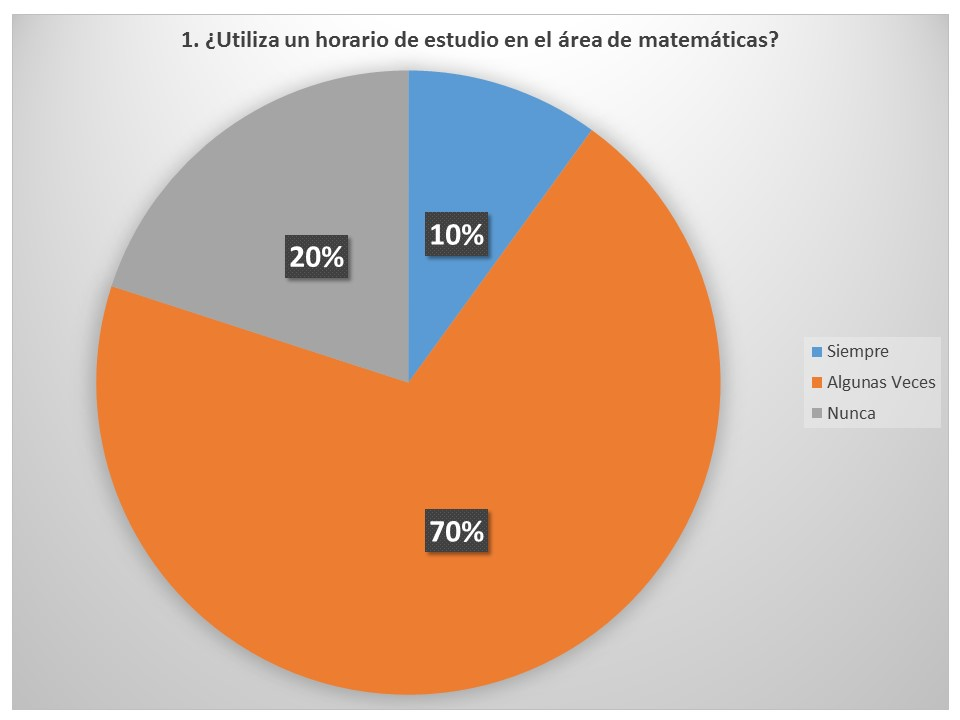
\includegraphics[scale=.7]{pregunta1.JPG}
\caption{Pregunta 1. ¿Utiliza un horario de estudio en el área de matemáticas?}
\end{figure}
\begin{figure}[H]
\centering
La siguiente tabla muestra el número de horas destinadas por un estudiante a realizar sus tareas de matemáticas, podemos observar que la que sobresale es de 1-3 hrs, debido a que la gran mayoría de los encuestados contesto que utilizaba ese promedio de horas.
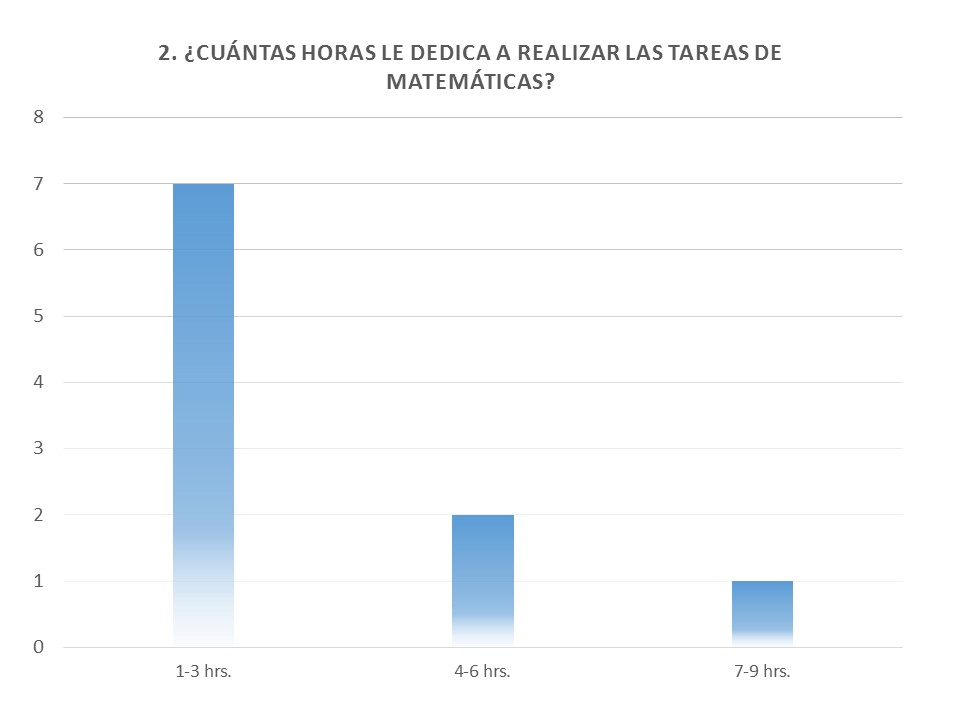
\includegraphics[scale=.7]{pregunta2.JPG}
\caption{Pregunta 2. ¿Cuántas horas le dedica a realizar las tareas de matemáticas?}
\end{figure}
\begin{figure}[H]
\centering
Lo que se puede observar en esta tabla es que la gran mayoría de los alumnos encuestados a reprobado alguna vez una materia de la asignatura de matemáticas.
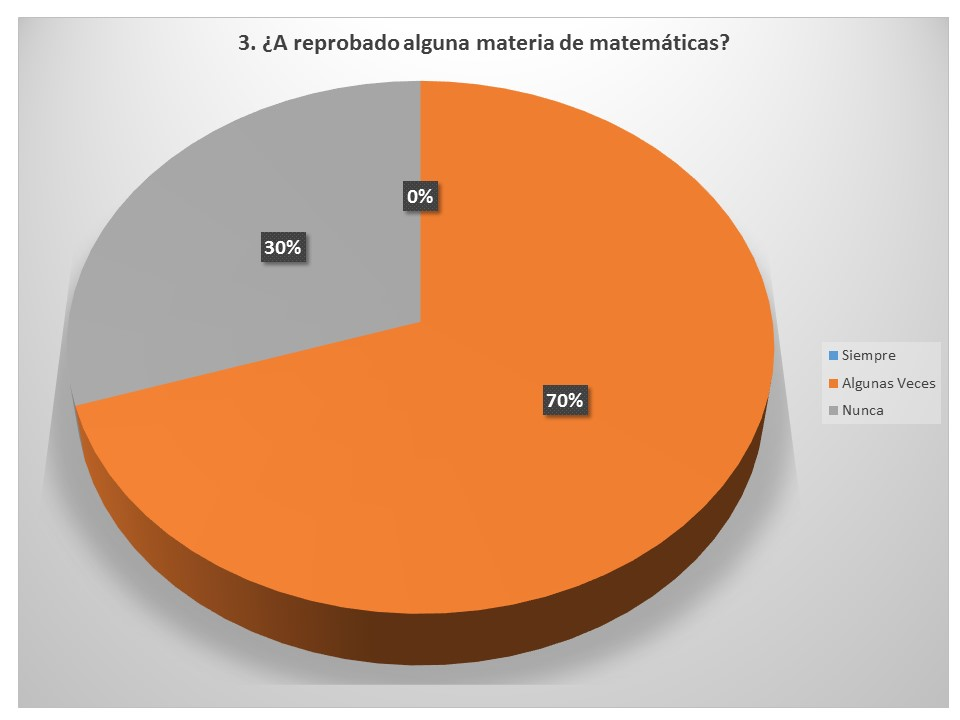
\includegraphics[scale=.7]{pregunta3.JPG}
\caption{Pregunta 3. ¿A reprobado alguna materia de matemáticas?}
\end{figure}
\begin{figure}[H]
\centering
Los datos arrojados por esta tabla es que un 80 por ciento de los estudiantes considerá que cuenta con un desempeño bueno en la materia de matemáticas y el otro 20 por ciento respondión que es excelente.
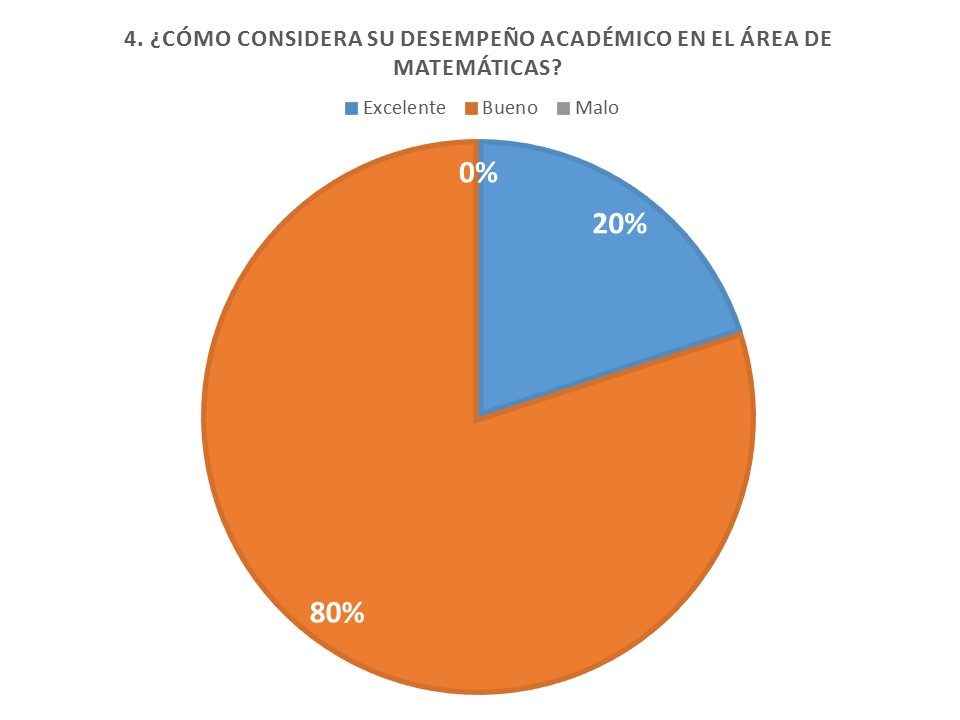
\includegraphics[scale=.7]{pregunta4.JPG}
\caption{Pregunta 4. ¿Cómo considera su desempeño académico en el área de matemáticas?}
\end{figure}
\begin{figure}[H]
\centering
En esta pregunta las respuestas fueron muy variadas, un 20 por ciento mencionó que nuca utiliza un horario para la asignatura de programación y un 40 por ciento contesto que siempre o algunas veces respectivamente.  
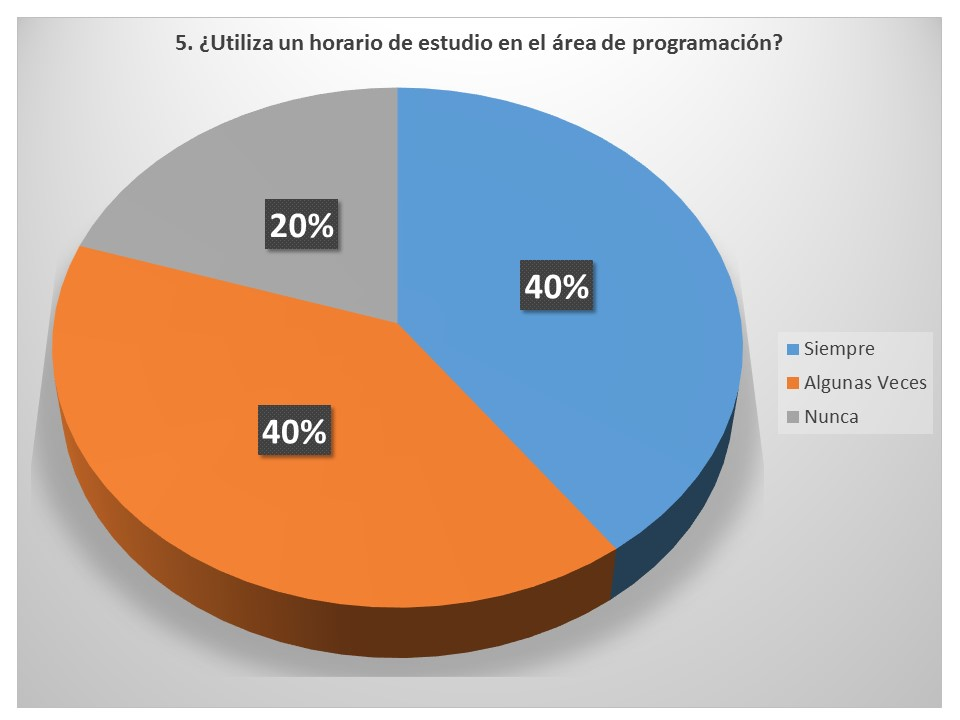
\includegraphics[scale=.7]{pregunta5.JPG}
\caption{Pregunta 5. ¿Utiliza un horario de estudio en el área de programación?}
\end{figure}
\begin{figure}[H]
\centering
Al igual que en la asignatura de matemáticas, la mayoría de los alumnos encuestados respondió que destina un promedio de 1 a 3 horas para realizar sus tareas de programación.  
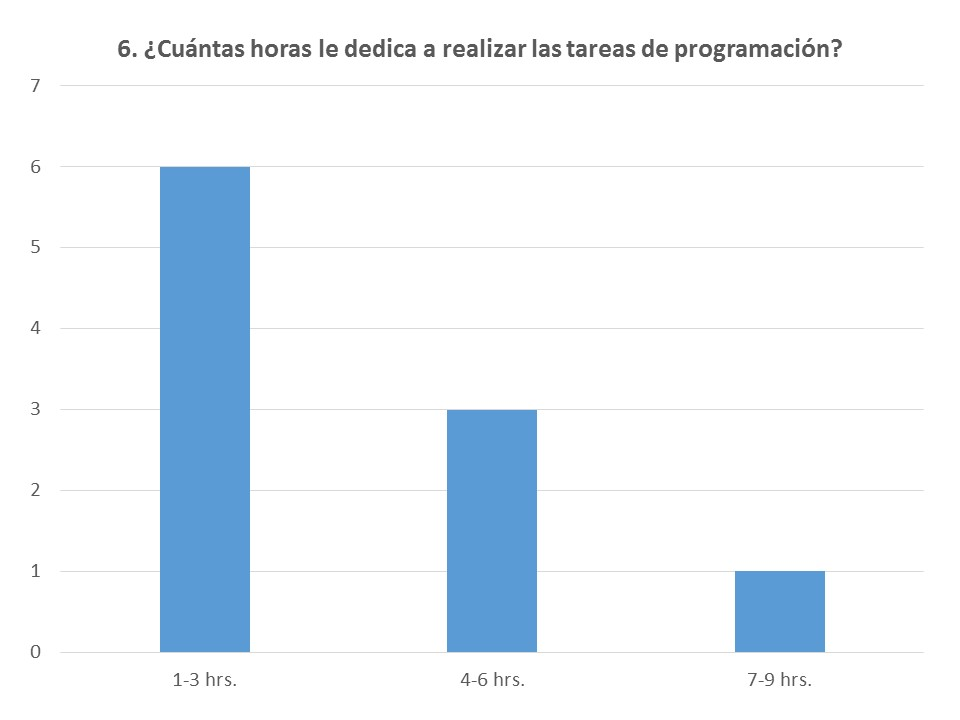
\includegraphics[scale=.7]{pregunta6.JPG}
\caption{Pregunta 6. ¿Cuántas horas le dedica a realizar las tareas de programación?}
\end{figure}
\begin{figure}[H]
\centering
En esta tabla podemos observar que un 60 por ciento de los estudiantes encuestados respondio que algunas veces ha reprobado una materia de programación y el otro 40 por ciento de los encuestados dijo nunca haber reprobado una de las materias de programación.   
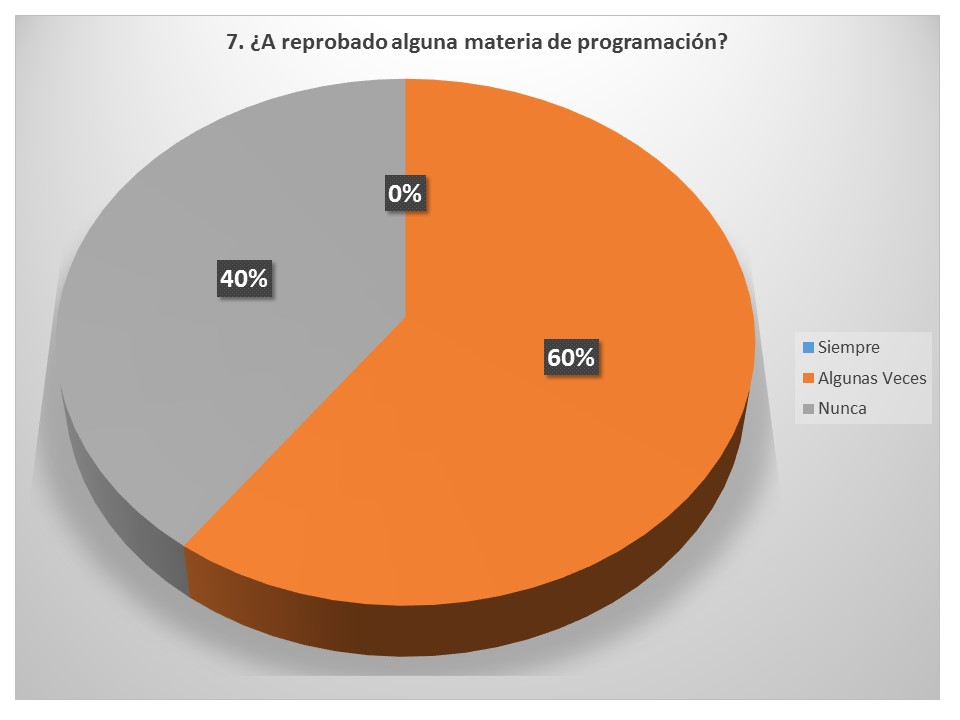
\includegraphics[scale=.7]{pregunta7.JPG}
\caption{Pregunta 7. ¿A reprobado alguna materia de programación?}
\end{figure}
\begin{figure}[H]
\centering
La gran mayoría respondió que su desempeño en las asignaturas relacionadas con programación ha sido bueno con un total de 7 alumnos y el restante comentó tener un desempeño malo.  
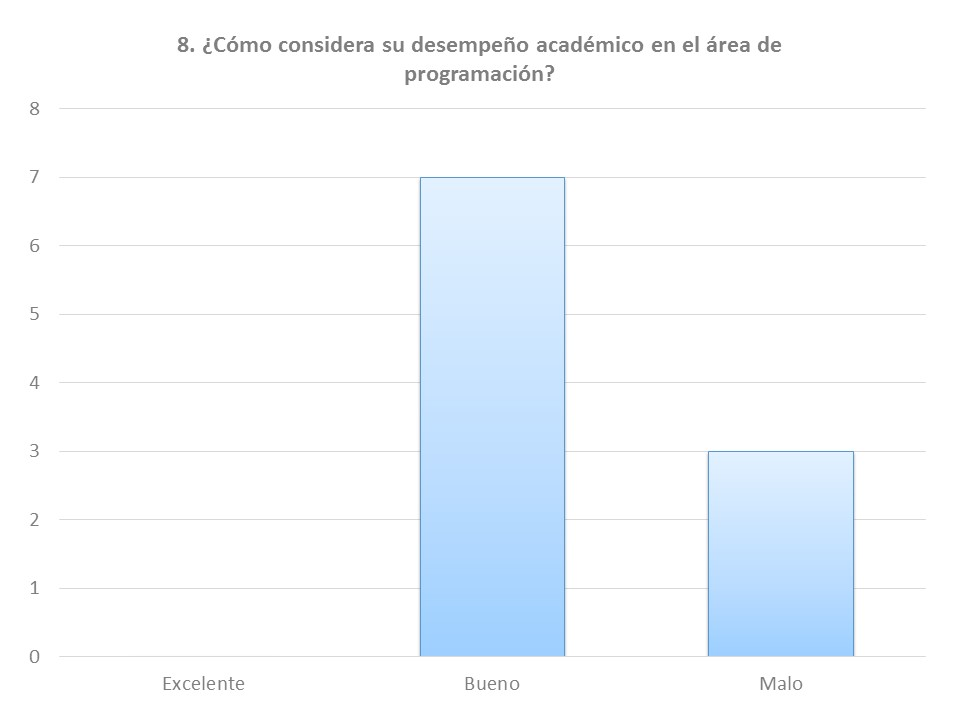
\includegraphics[scale=.7]{pregunta8.JPG}
\caption{Pregunta 8. ¿Cómo considera su desempeño académico en el área de programación?}
\end{figure}
A continuación se muestran las gráficas de los resultados obtenidos por los alumnos en la aplicación del examen de programación.\\
\begin{figure}[H]
\centering 
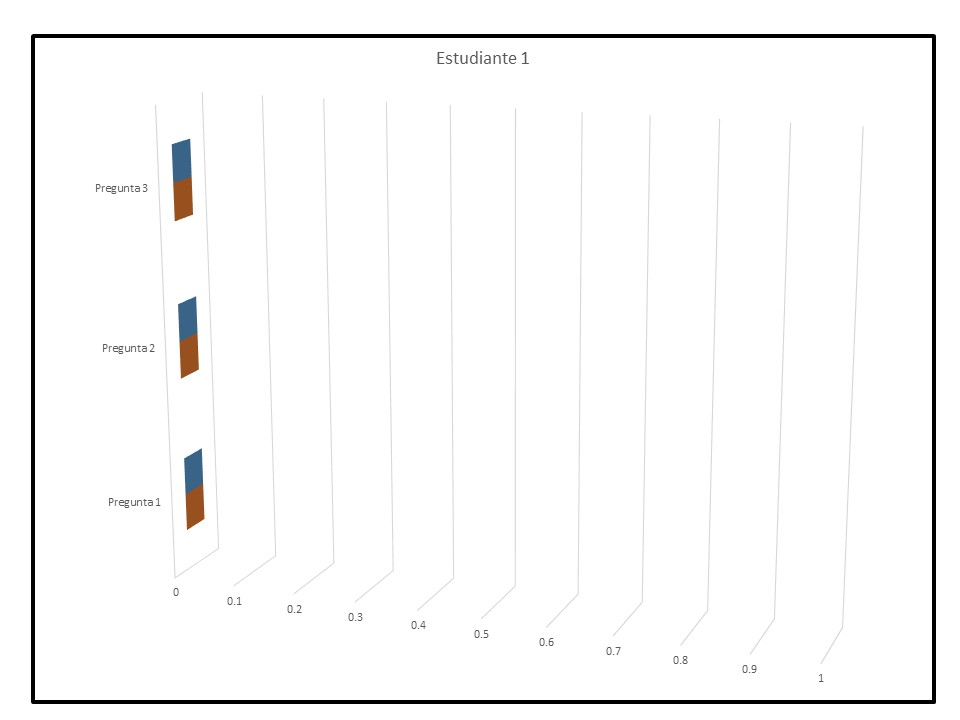
\includegraphics[scale=.7]{PEstudiante1.JPG}
\caption{Resultados obtenidos por un alumno en el examen de programación}
\end{figure}

\begin{figure}[H]
\centering 
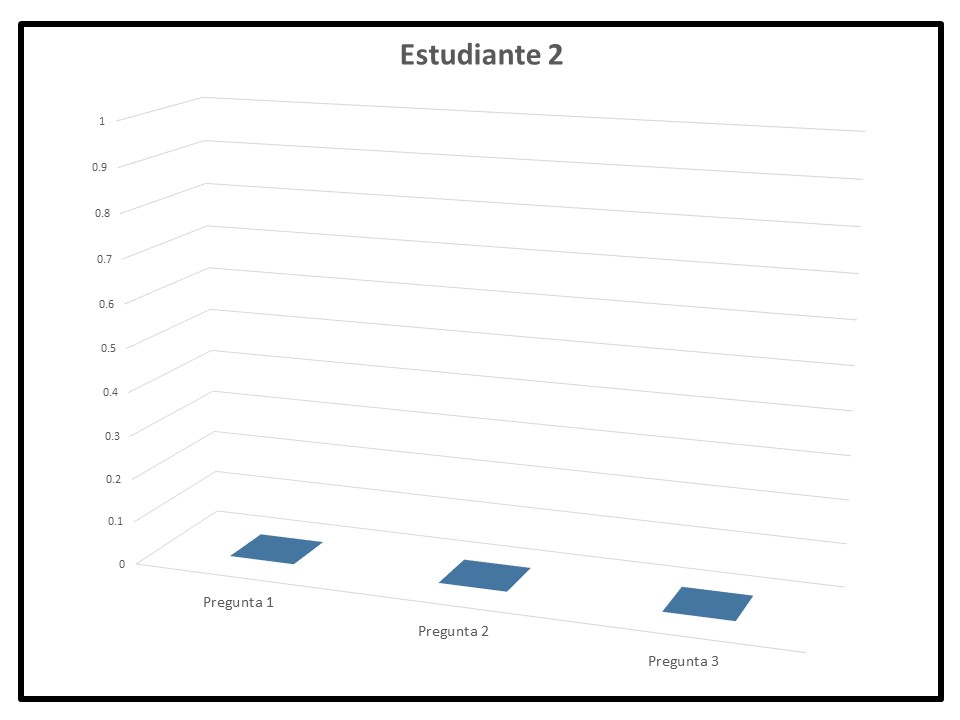
\includegraphics[scale=.7]{PEstudiante2.JPG}
\caption{Resultados obtenidos por un alumno en el examen de programación}
\end{figure}

\begin{figure}[H]
\centering 
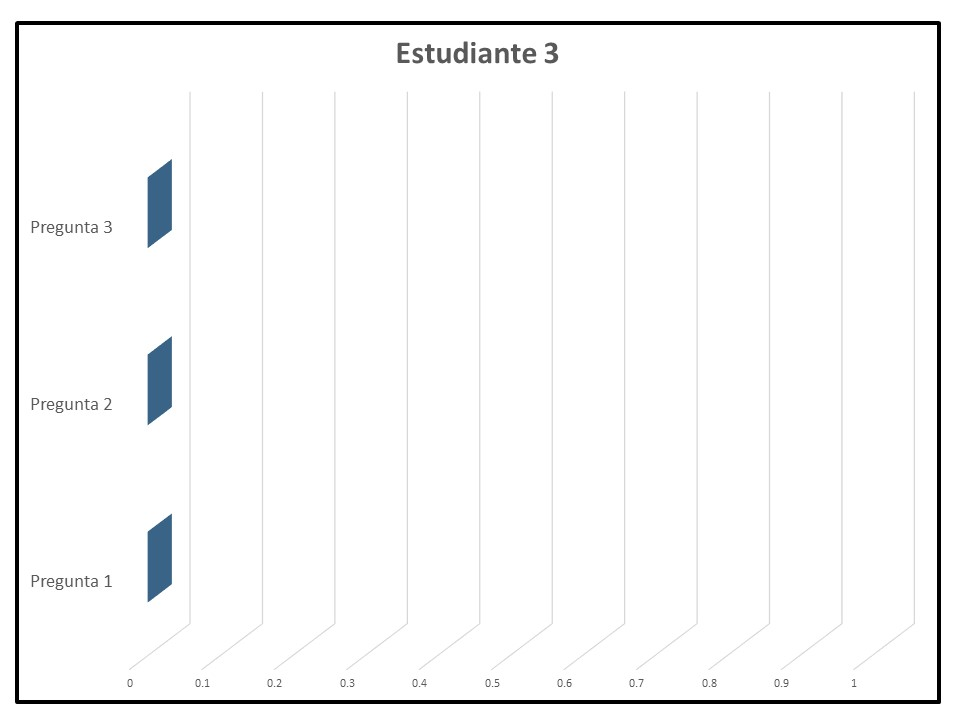
\includegraphics[scale=.7]{PEstudiante3.JPG}
\caption{Resultados obtenidos por un alumno en el examen de programación}
\end{figure}

\begin{figure}[H]
\centering 
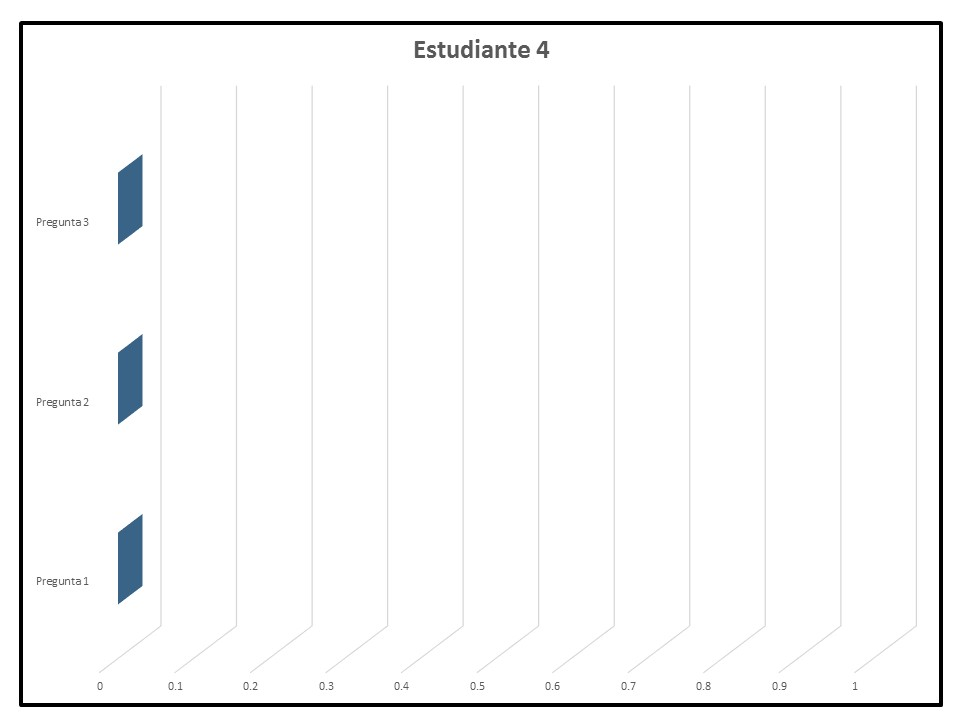
\includegraphics[scale=.7]{PEstudiante4.JPG}
\caption{Resultados obtenidos por un alumno en el examen de programación}
\end{figure}

\begin{figure}[H]
\centering 
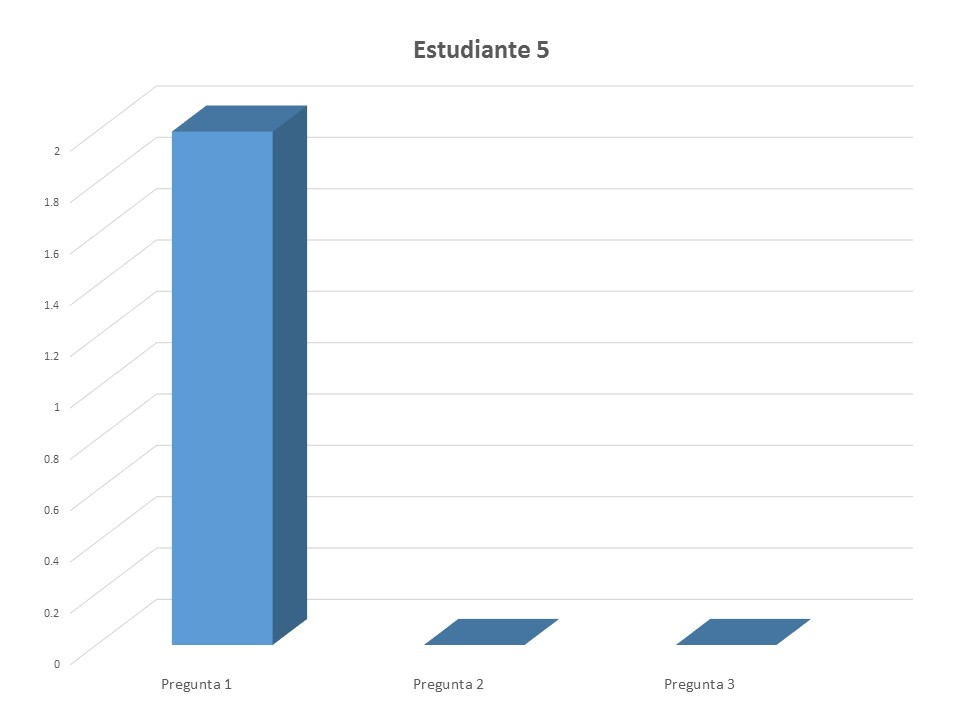
\includegraphics[scale=.7]{PEstudiante5.JPG}
\caption{Resultados obtenidos por un alumno en el examen de programación}
\end{figure}

\begin{figure}[H]
\centering 
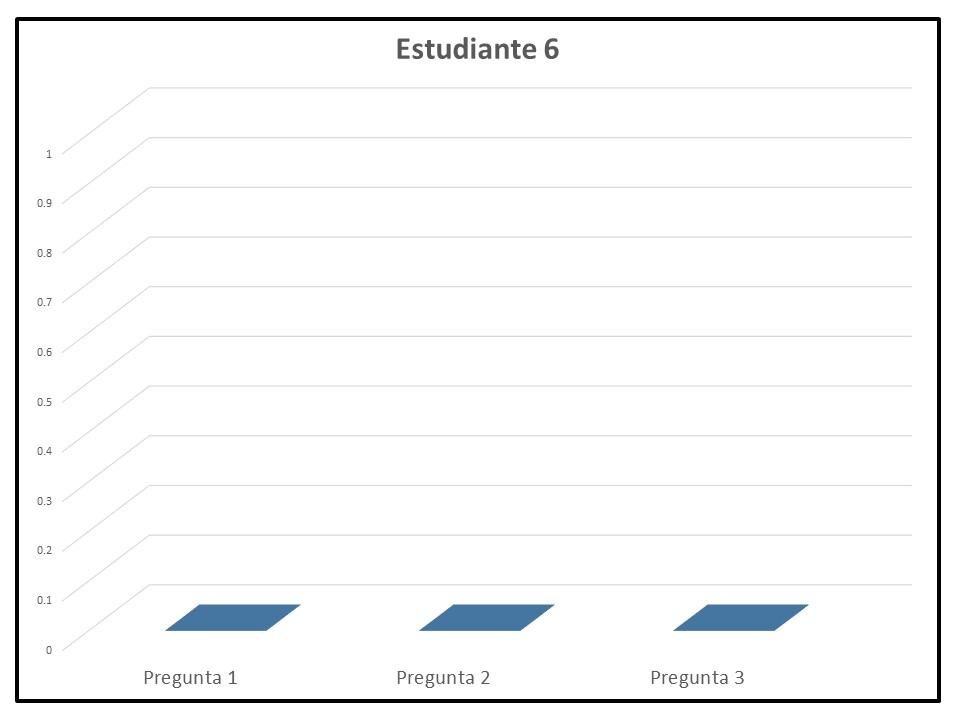
\includegraphics[scale=.7]{PEstudiante6.JPG}
\caption{Resultados obtenidos por un alumno en el examen de programación}
\end{figure}

\begin{figure}[H]
\centering 
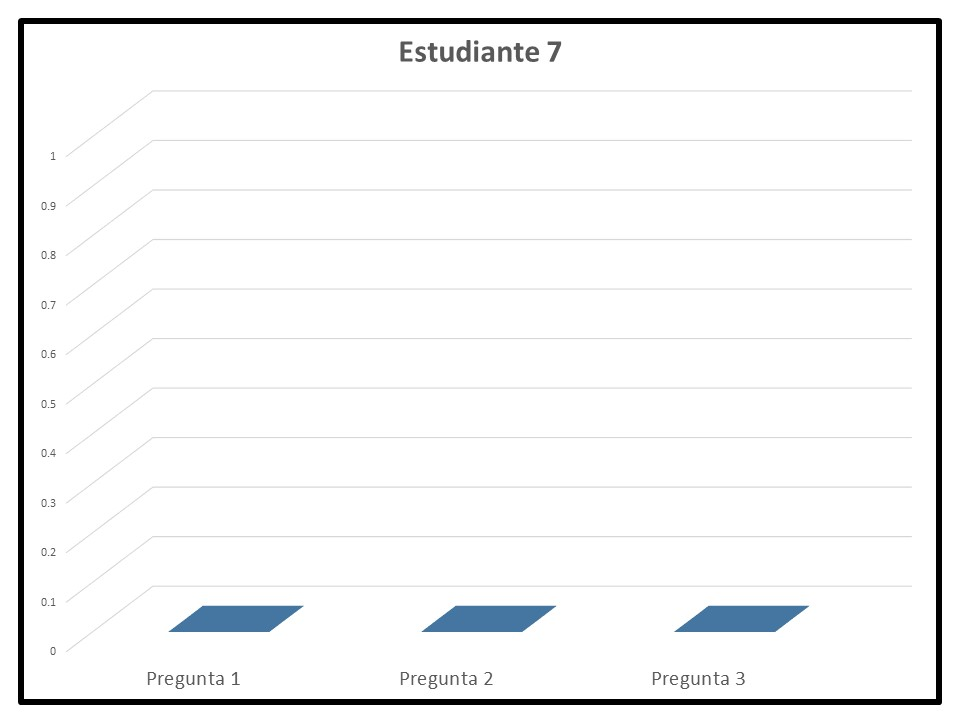
\includegraphics[scale=.7]{PEstudiante7.JPG}
\caption{Resultados obtenidos por un alumno en el examen de programación}
\end{figure}

\begin{figure}[H]
\centering 
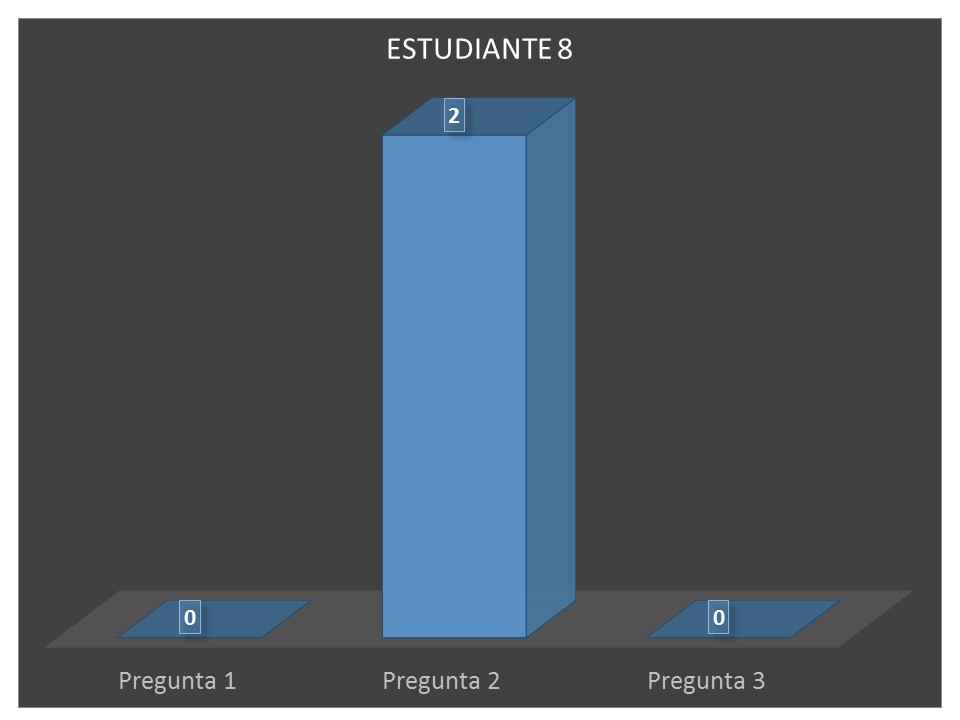
\includegraphics[scale=.7]{PEstudiante8.JPG}
\caption{Resultados obtenidos por un alumno en el examen de programación}
\end{figure}

\begin{figure}[H]
\centering 
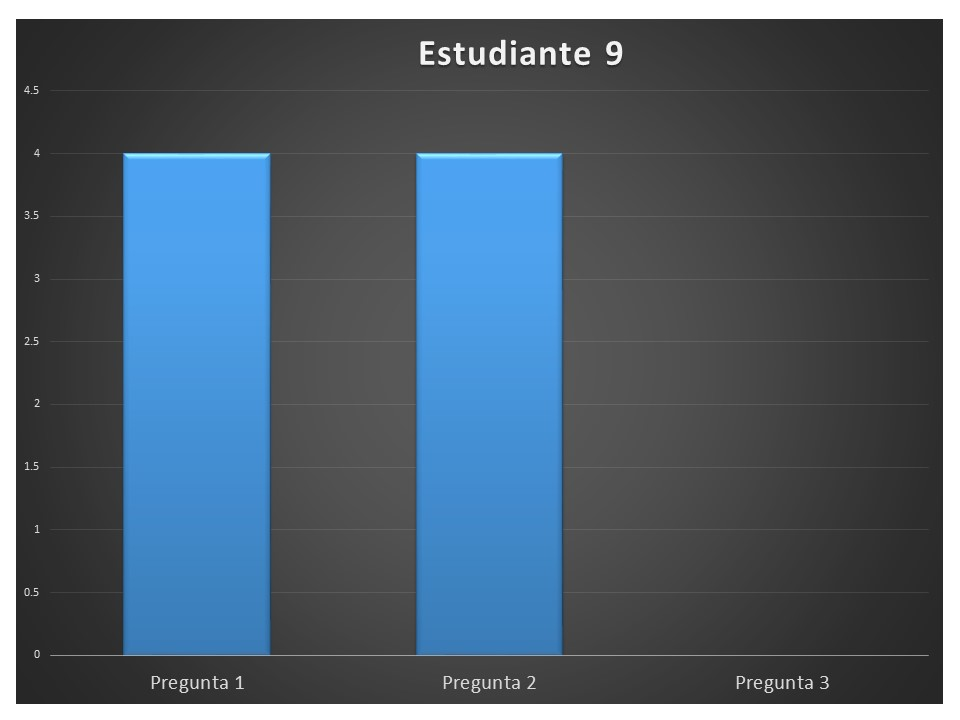
\includegraphics[scale=.7]{PEstudiante9.JPG}
\caption{Resultados obtenidos por un alumno en el examen de programación}
\end{figure}

\begin{figure}[H]
\centering 
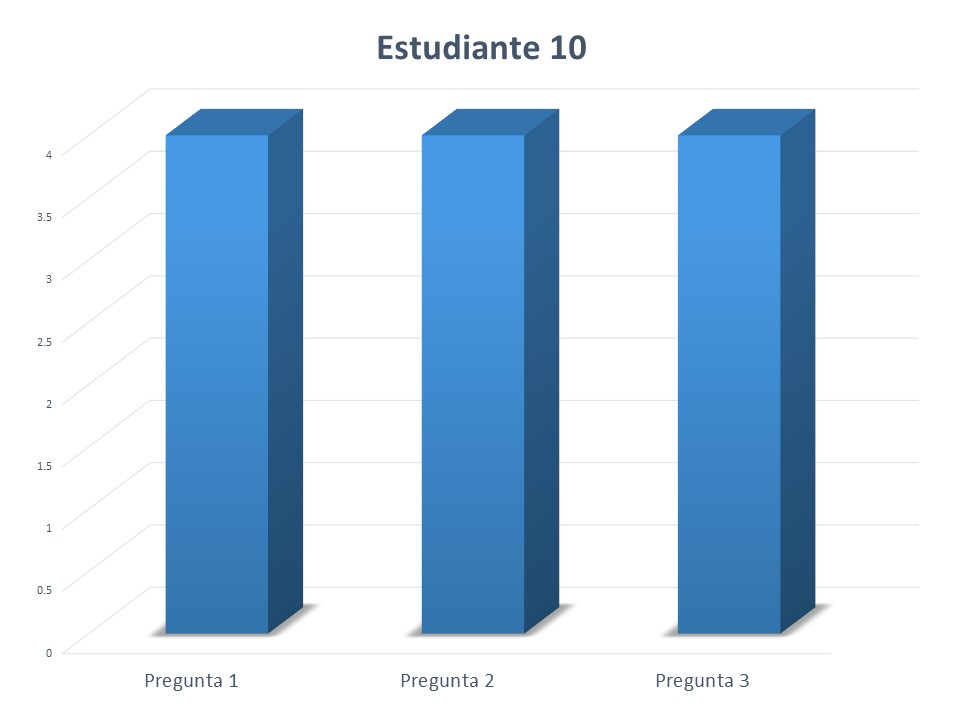
\includegraphics[scale=.7]{PEstudiante10.JPG}
\caption{Resultados obtenidos por un alumno en el examen de programación}
\end{figure}

Las gráficas que se muestran a continuación reflejan los resultados obtenidos por los alumnos en la aplicación del exámen de matemáticas(Resolución de ecuaciones lineales).//

\begin{figure}[H]
\centering 
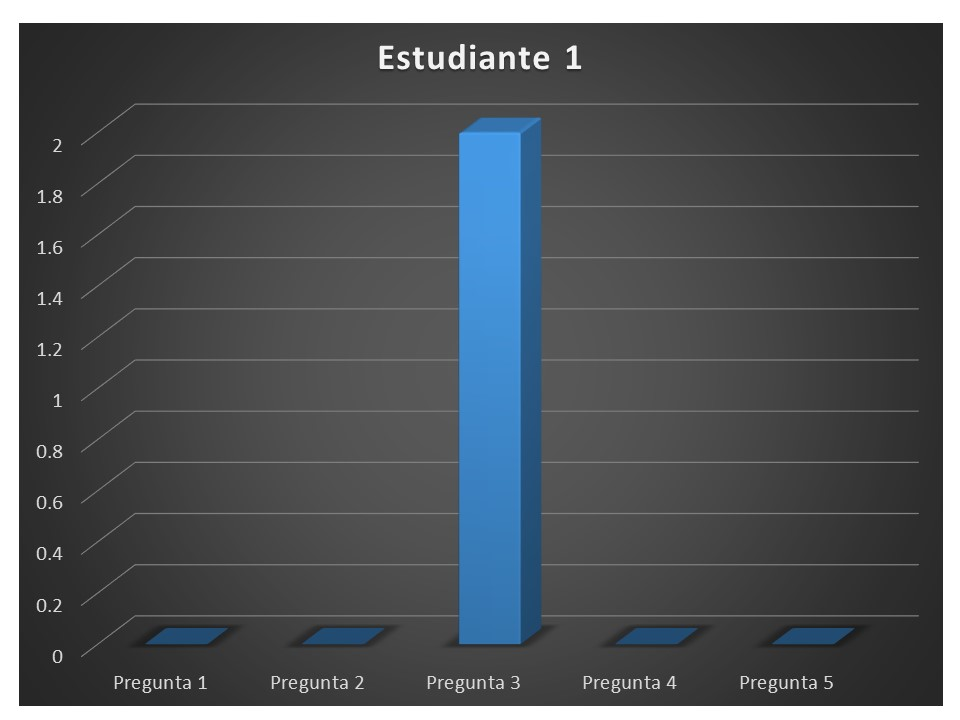
\includegraphics[scale=.7]{MEstudiante1.JPG}
\caption{Resultados obtenidos por un alumno en el examen de matemáticas}
\end{figure}

\begin{figure}[H]
\centering 
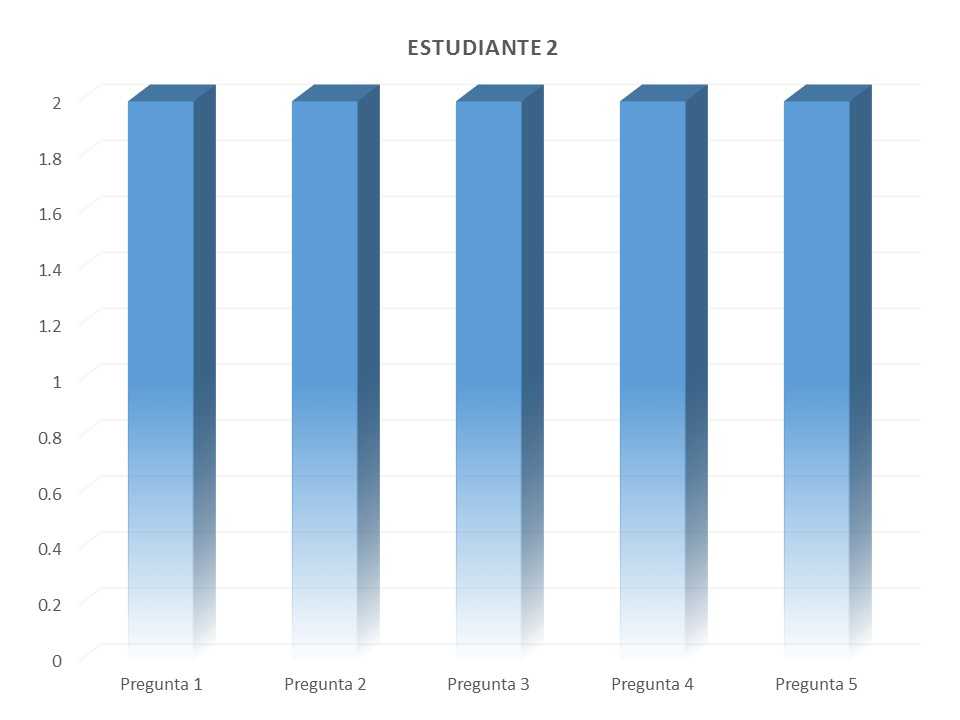
\includegraphics[scale=.7]{MEstudiante2.JPG}
\caption{Resultados obtenidos por un alumno en el examen de matemáticas}
\end{figure}
\begin{figure}[H]
\centering 
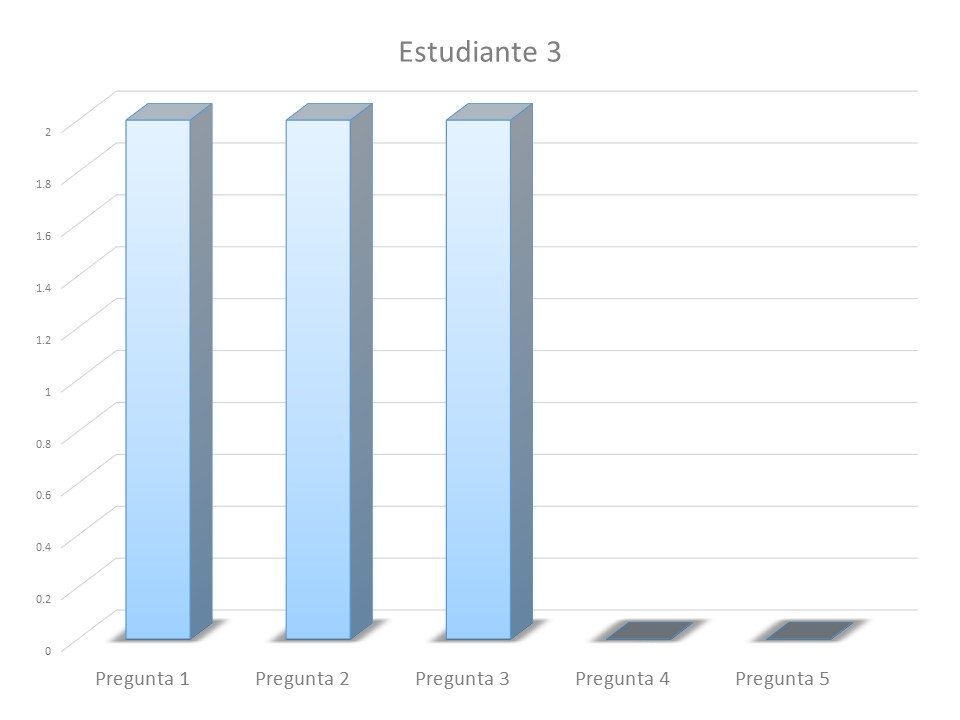
\includegraphics[scale=.7]{MEstudiante3.JPG}
\caption{Resultados obtenidos por un alumno en el examen de matemáticas}
\end{figure}
\begin{figure}[H]
\centering 
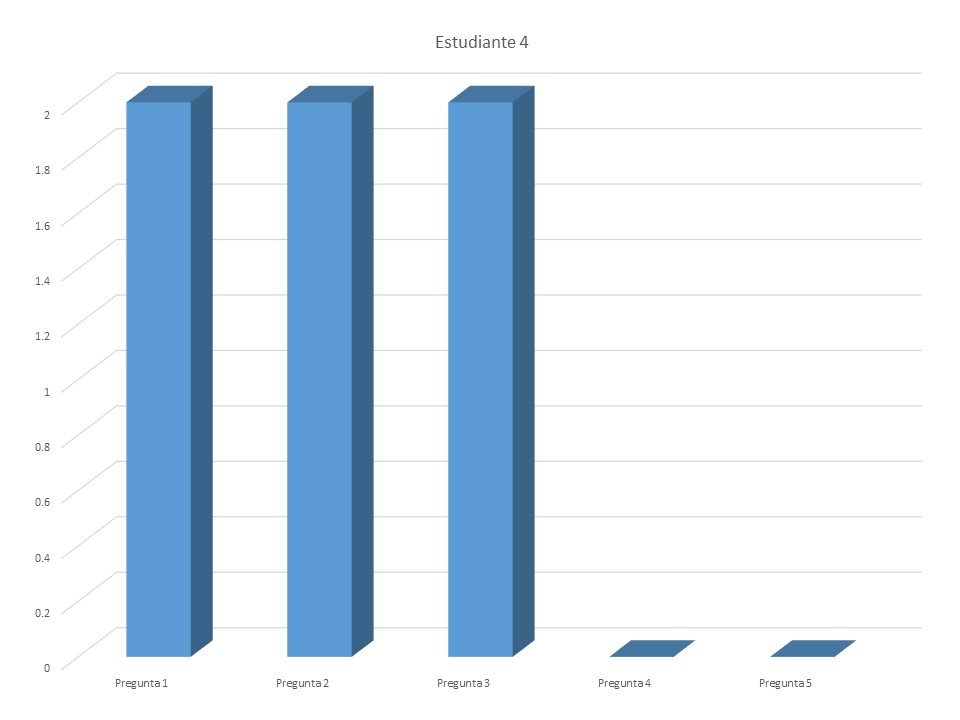
\includegraphics[scale=.7]{MEstudiante4.JPG}
\caption{Resultados obtenidos por un alumno en el examen de matemáticas}
\end{figure}
\begin{figure}[H]
\centering 
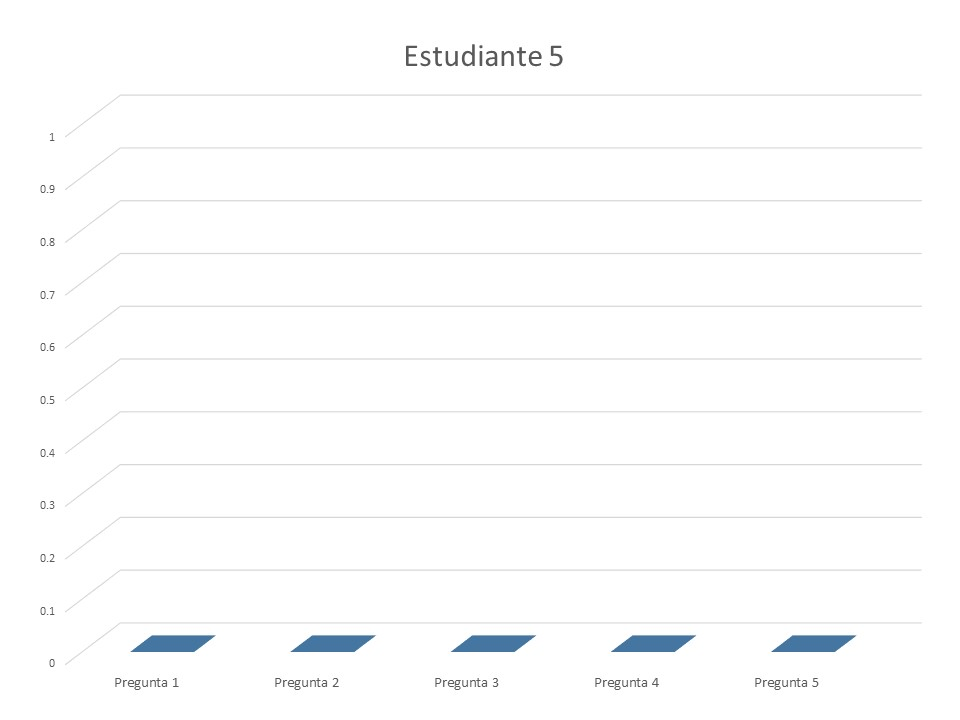
\includegraphics[scale=.7]{MEstudiante5.JPG}
\caption{Resultados obtenidos por un alumno en el examen de matemáticas}
\end{figure}
\begin{figure}[H]
\centering 
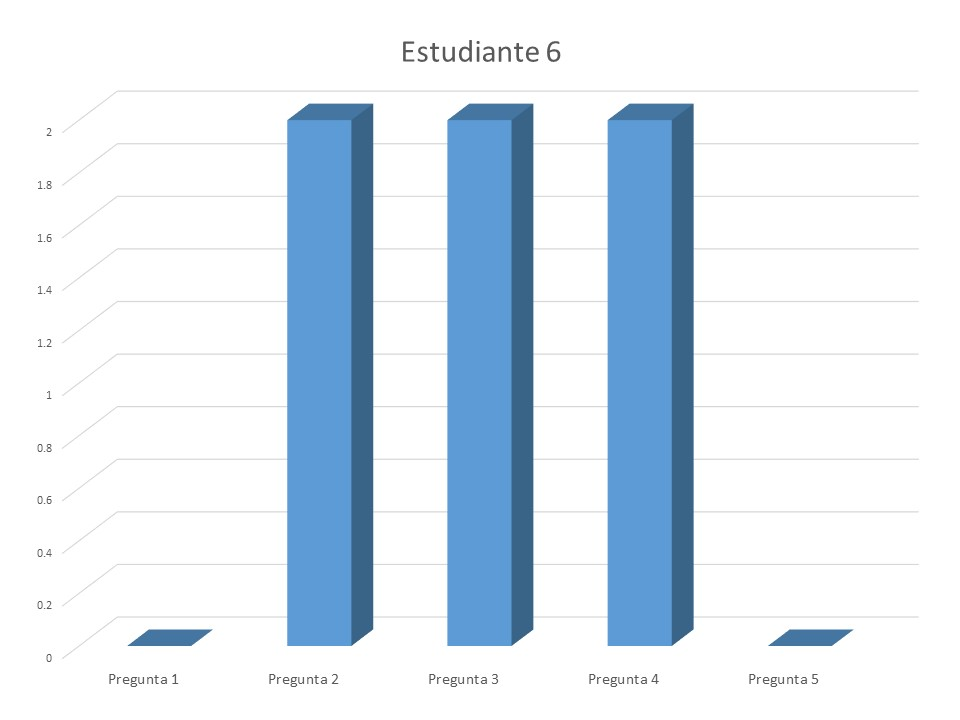
\includegraphics[scale=.7]{MEstudiante6.JPG}
\caption{Resultados obtenidos por un alumno en el examen de matemáticas}
\end{figure}
\begin{figure}[H]
\centering 
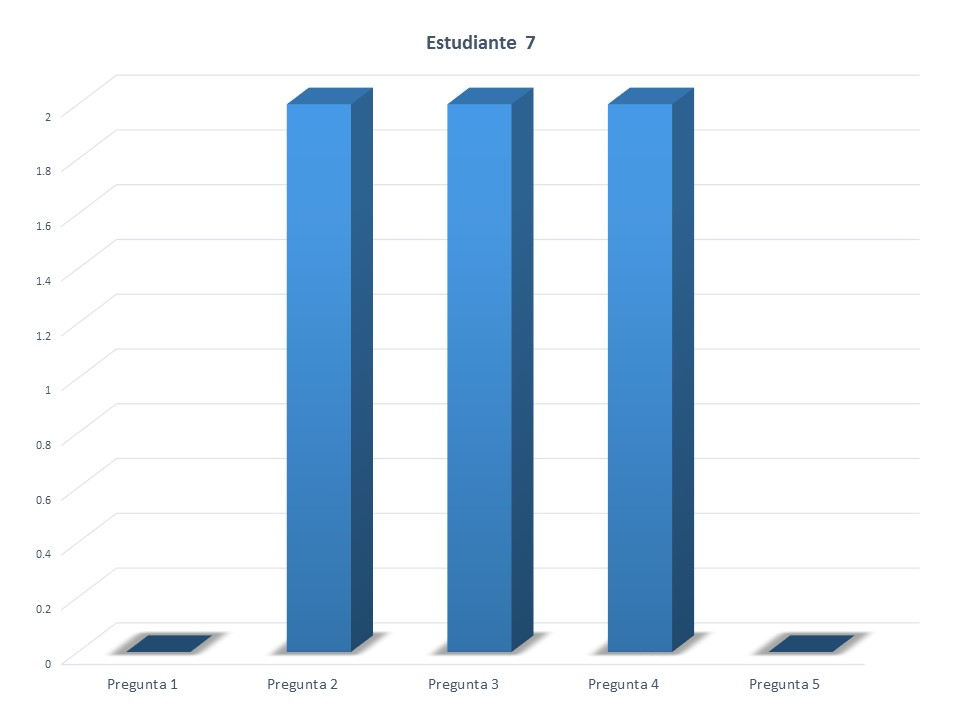
\includegraphics[scale=.7]{MEstudiante7.JPG}
\caption{Resultados obtenidos por un alumno en el examen de matemáticas}
\end{figure}
\begin{figure}[H]
\centering 
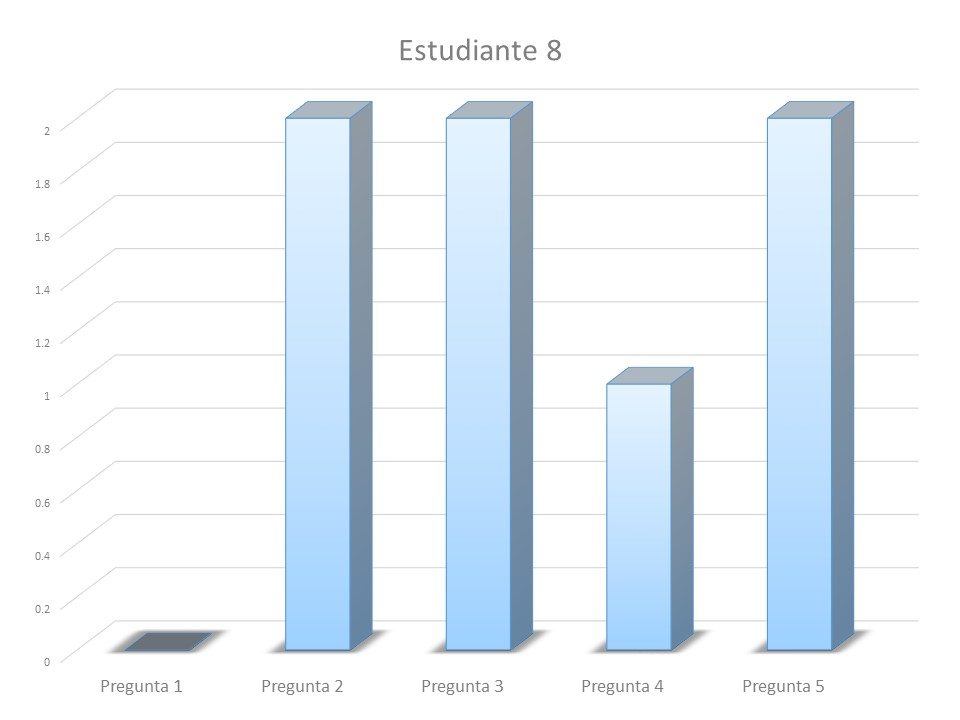
\includegraphics[scale=.7]{MEstudiante8.JPG}
\caption{Resultados obtenidos por un alumno en el examen de matemáticas}
\end{figure}
\begin{figure}[H]
\centering 
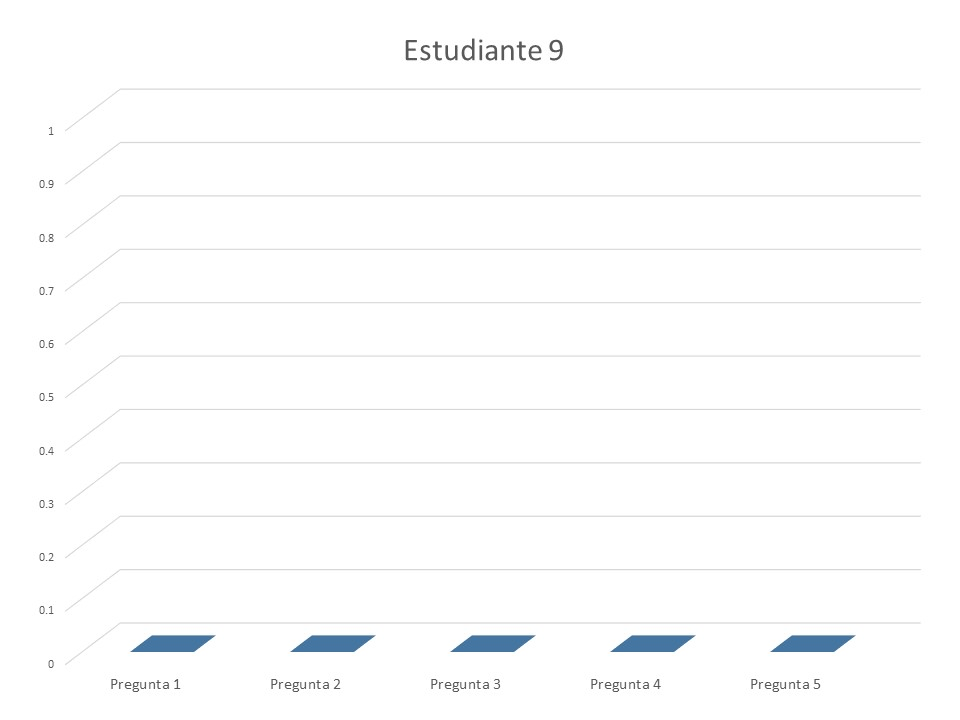
\includegraphics[scale=.7]{MEstudiante9.JPG}
\caption{Resultados obtenidos por un alumno en el examen de matemáticas}
\end{figure}
\begin{figure}[H]
\centering 
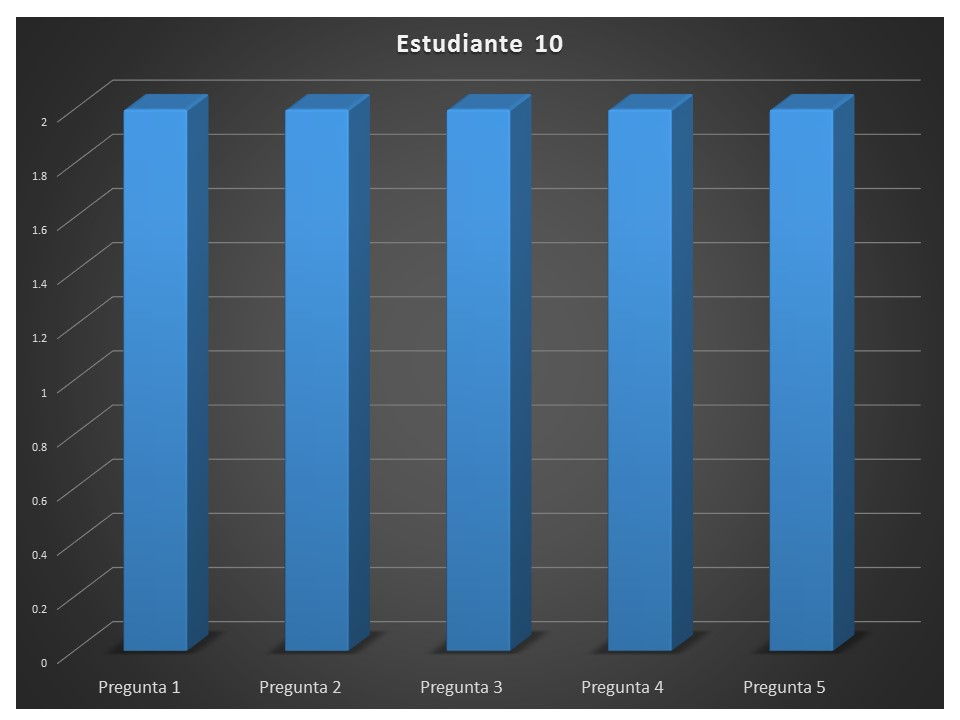
\includegraphics[scale=.7]{MEstudiante10.JPG}
\caption{Resultados obtenidos por un alumno en el examen de matemáticas}
\end{figure}


\section{Índices de correlación entre variables}
A continuación se mostrarán una serie de tablas de las preguntas que obtuvieron un mayor número de correlación en la aplicación de la encuesta:
\begin{figure}[H]
\centering 
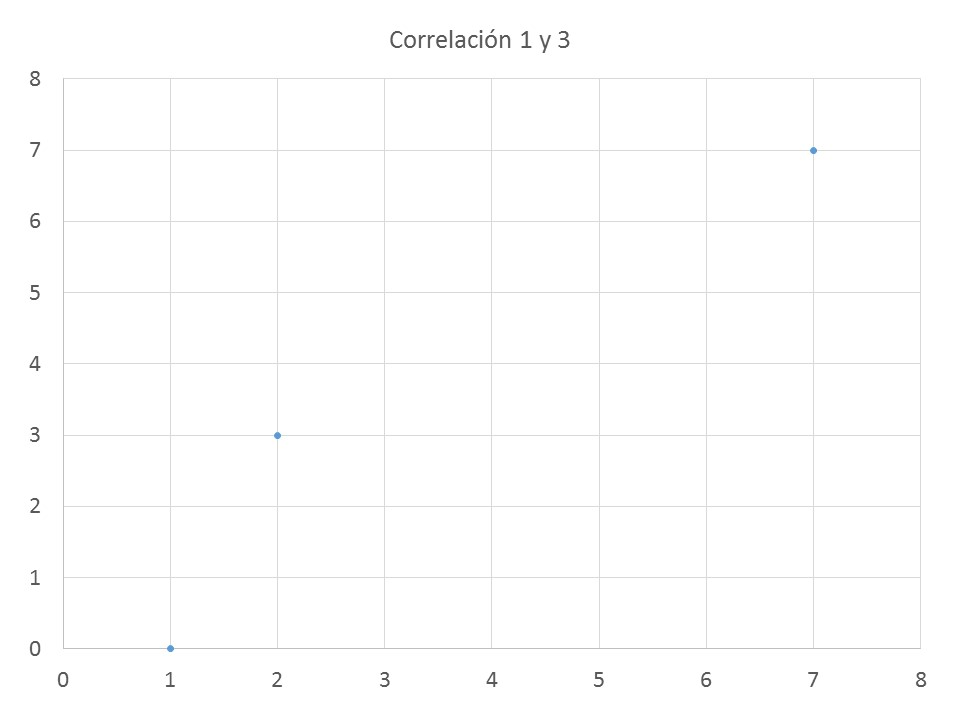
\includegraphics[scale=.7]{correlacion13.jpg}
\caption{Índice de correlación entre la pregunta 1 y la pregunta 3}
\end{figure}
\begin{figure}[H]
\centering 
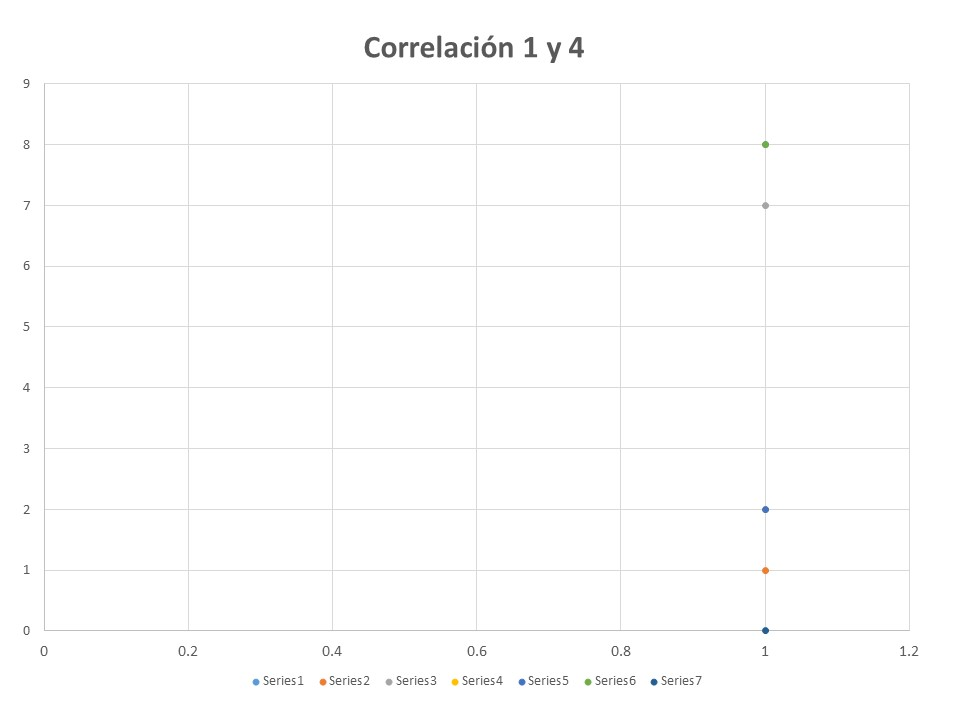
\includegraphics[scale=.7]{correlacion_14.jpg}
\caption{Índice de correlación entre la pregunta 1 y la pregunta 4}
\end{figure}
\begin{figure}[H]
\centering 
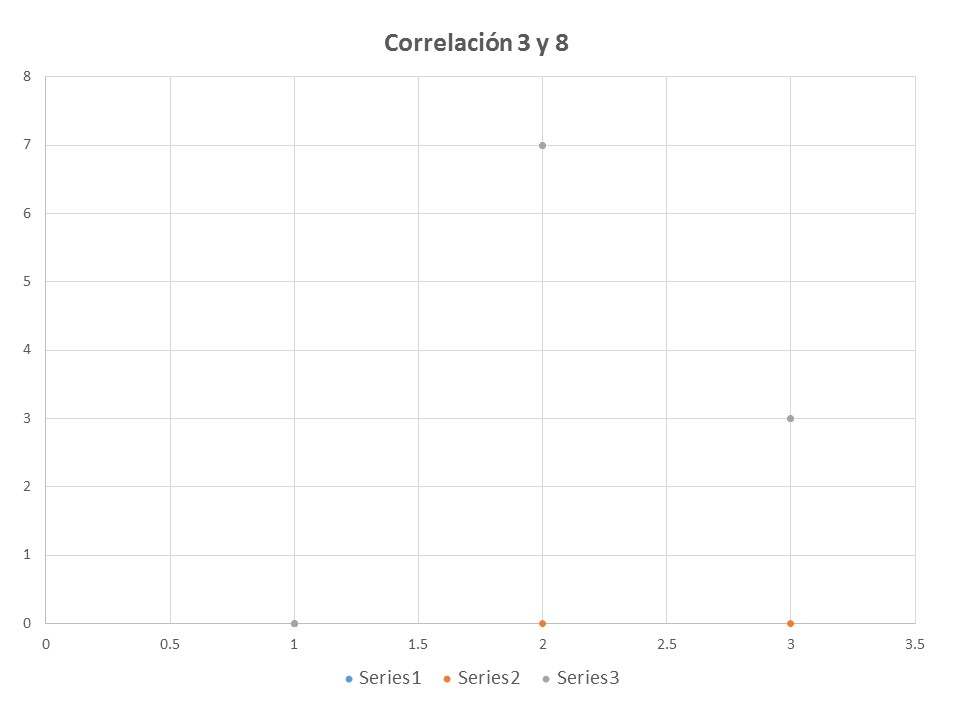
\includegraphics[scale=.7]{correlaci_n_38.jpg}
\caption{Índice de correlación entre la pregunta 3 y la pregunta 8}
\end{figure}
A continuación se muestra la tabla con mayor número de correlación en el examen de programación aplicado a los estudiantes de la carrera de ingeniería en sistemas.\\

\begin{figure}[H]
\centering 
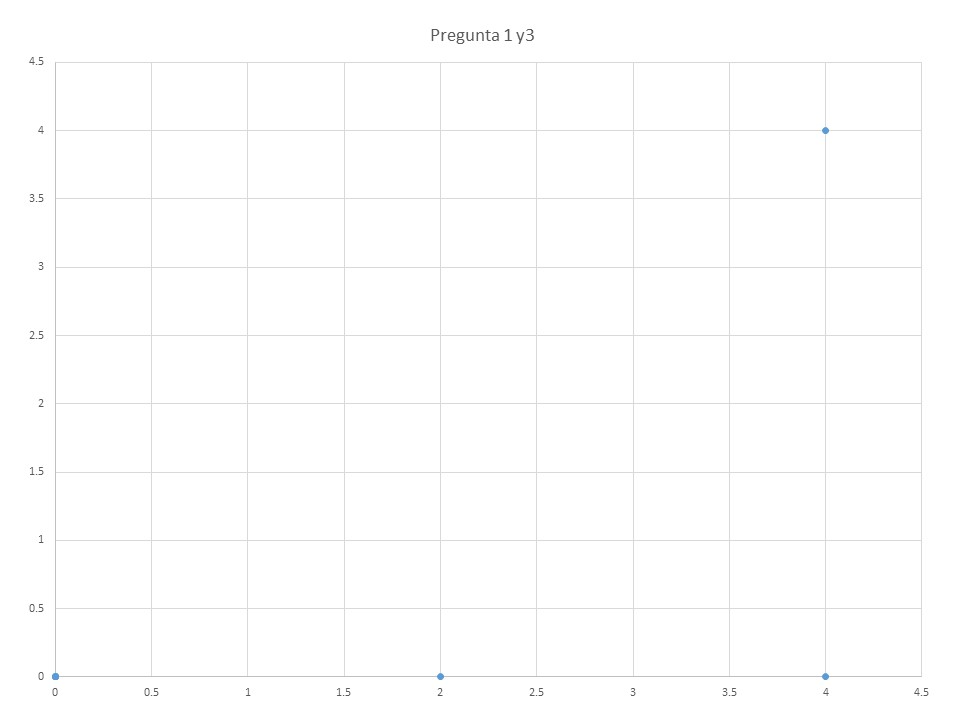
\includegraphics[scale=.7]{PCorrelacion1.jpg}
\caption{Índice de correlación entre la pregunta 1 y la pregunta 3}
\end{figure}

Ahora se muestran las preguntas que tuvieron mayor coeficiente de correlación en el exámen de matemáticas (Resolución de ecuaciones)

\begin{figure}[H]
\centering 
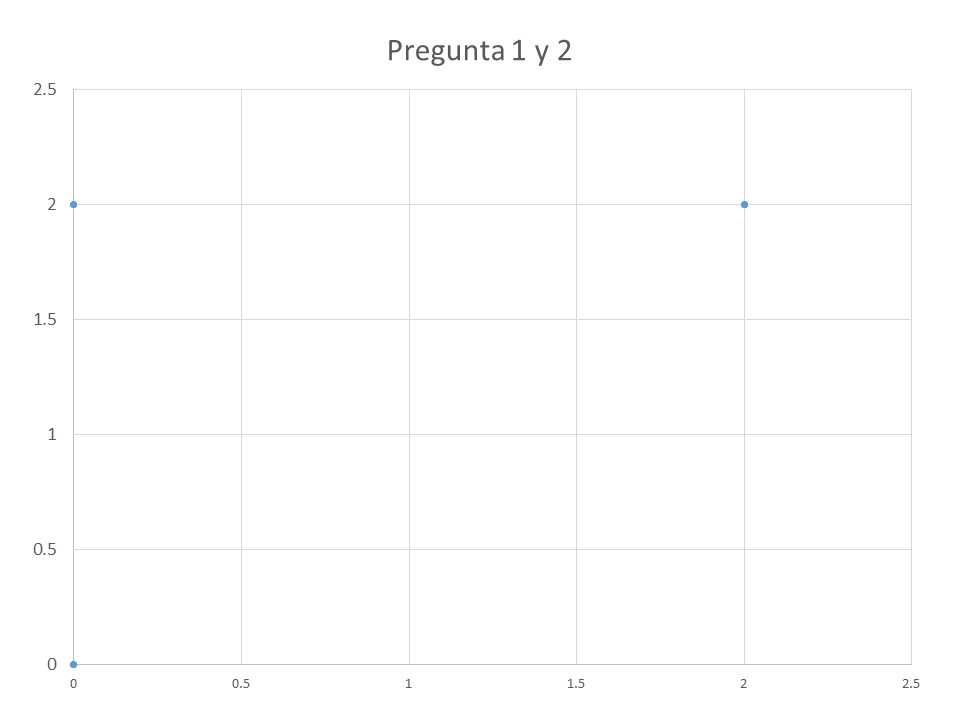
\includegraphics[scale=.7]{MCorrelacionmax12.JPG}
\caption{Índice de correlación entre la pregunta 1 y la pregunta 2}
\end{figure}

\begin{figure}[H]
\centering 
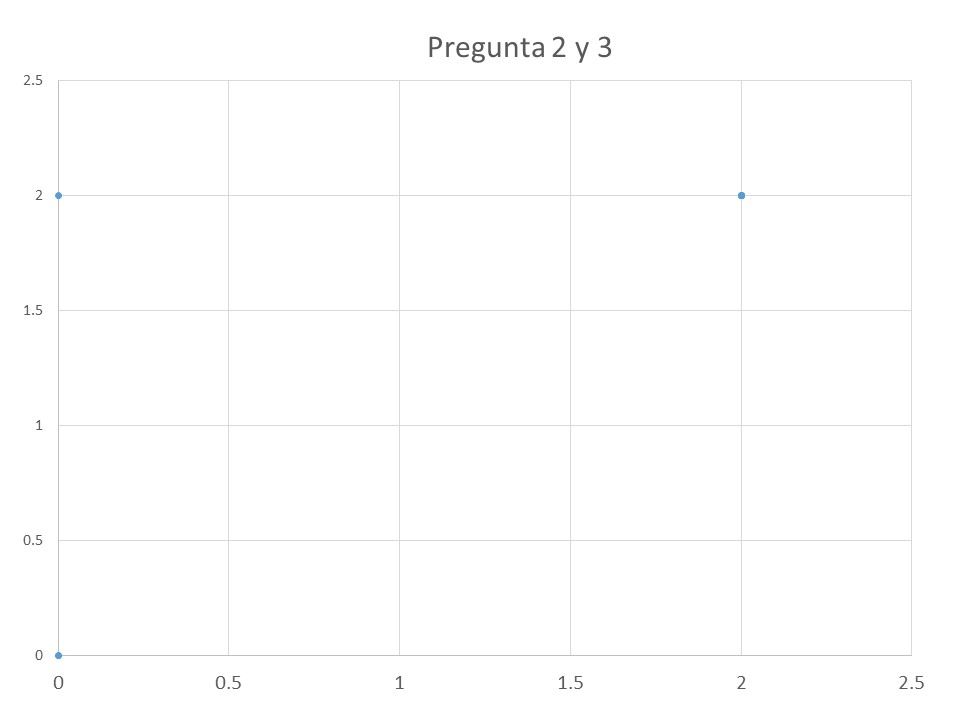
\includegraphics[scale=.7]{MCorrelacionmax23.JPG}
\caption{Índice de correlación entre la pregunta 2 y la pregunta 3}
\end{figure}

\begin{figure}[H]
\centering 
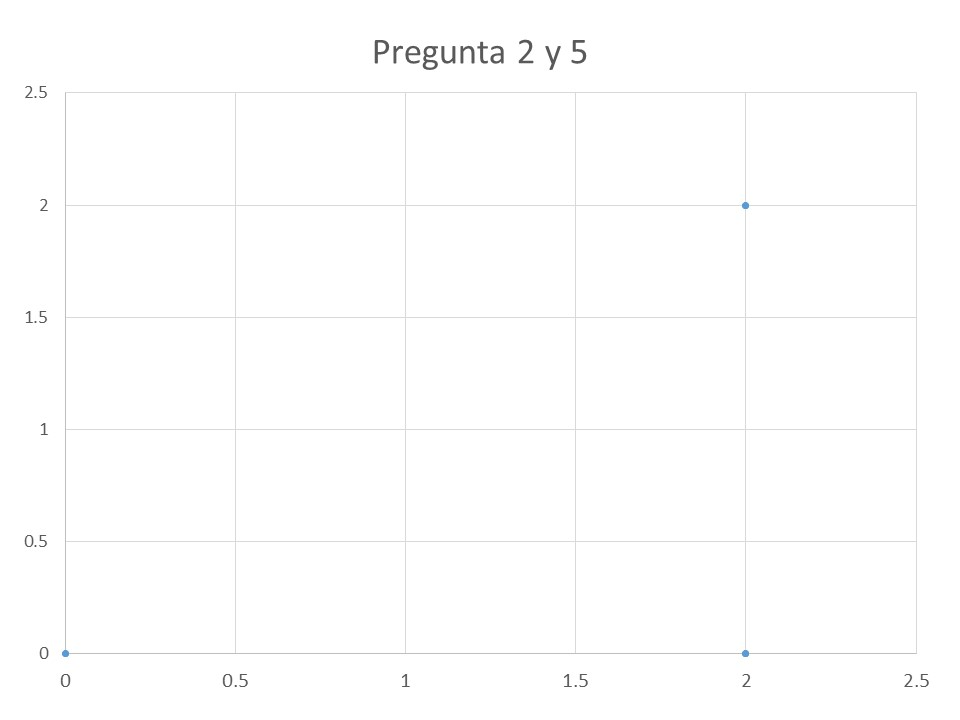
\includegraphics[scale=.7]{MCorrelacionmax25.JPG}
\caption{Índice de correlación entre la pregunta 2 y la pregunta 5}
\end{figure}
Las preguntas que obtuvieron menor coeficiente de correlación en la aplicación del exámen de matemáticas son las siguientes:
\begin{figure}[H]
\centering 
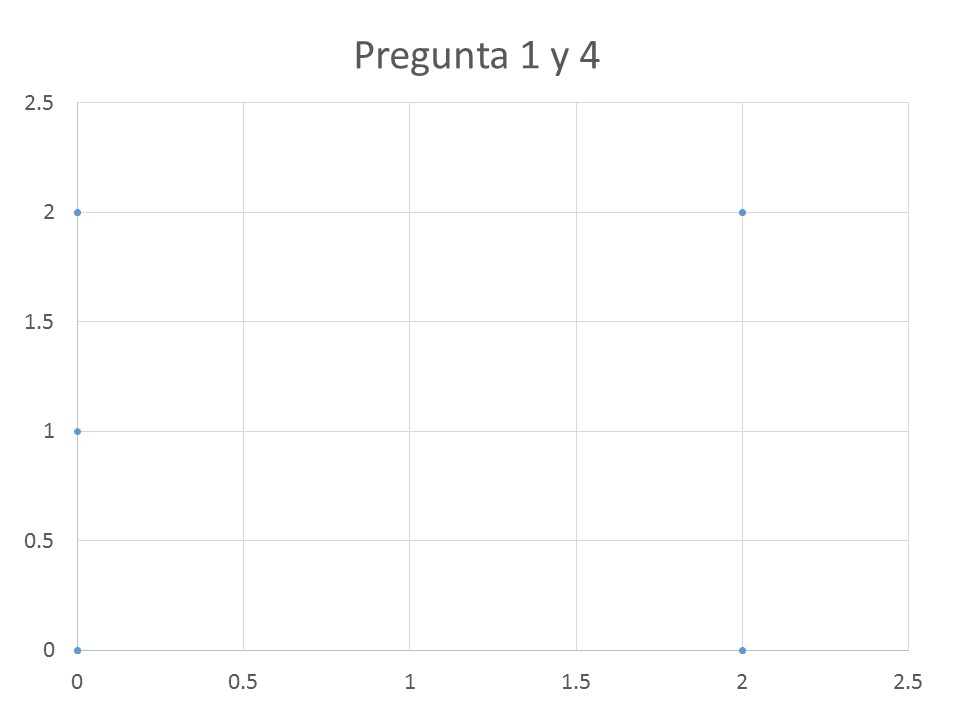
\includegraphics[scale=.7]{MCorrelacionmin14.JPG}
\caption{Índice de correlación entre la pregunta 1 y la pregunta 4}
\end{figure}

\begin{figure}[H]
\centering 
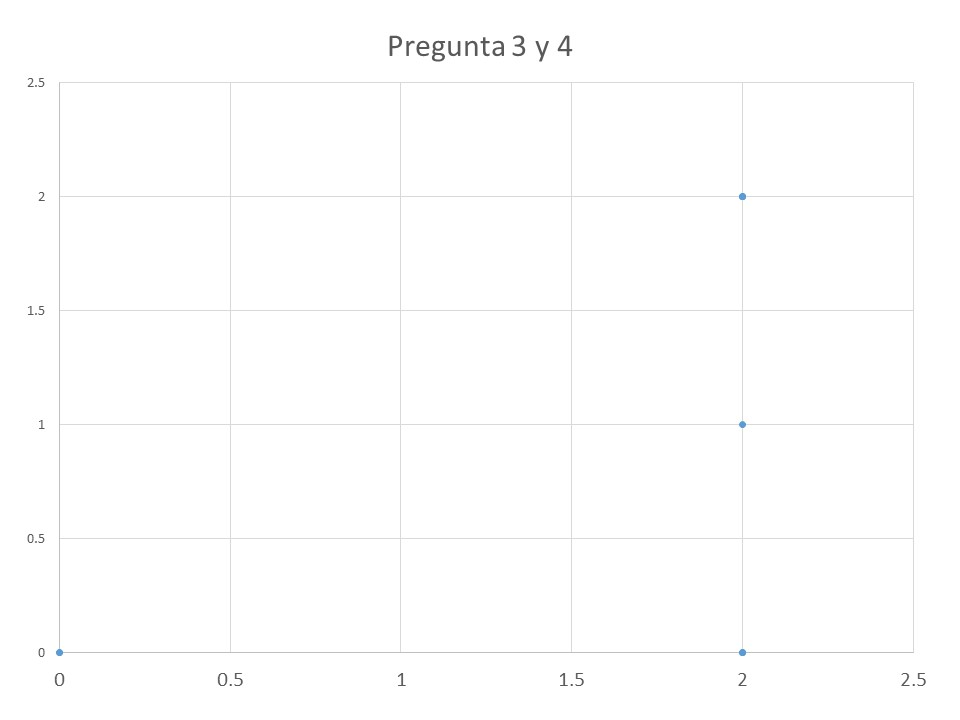
\includegraphics[scale=.7]{MCorrelacionmin34.JPG}
\caption{Índice de correlación entre la pregunta 3 y la pregunta 4}
\end{figure}

\begin{figure}[H]
\centering 
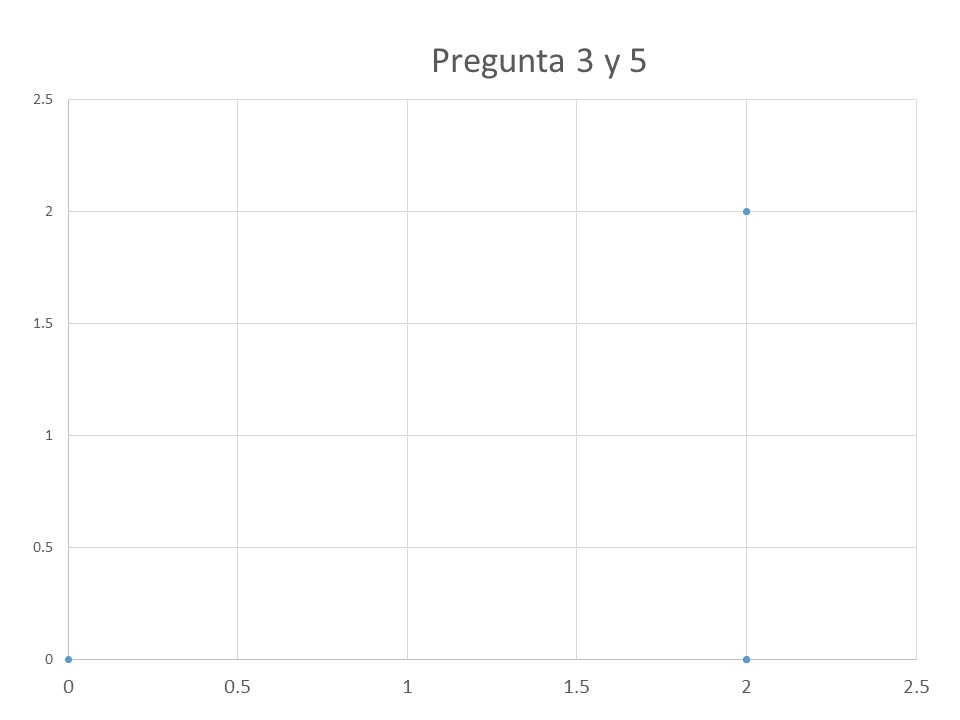
\includegraphics[scale=.7]{MCorrelacionmin35.JPG}
\caption{Índice de correlación entre la pregunta 3 y la pregunta 5}
\end{figure}

\section{Prueba de hipótesis}
Después de aplicar los instrumentos de evaluación a los estudiantes e interpretar la información obtenida con la generación de las gráficas de distribución de probabilidad, así como también el índice de correlación, la hipótesis planteada al principio de la investigación es declarada como falsa debido a que se observó que los que poseían habilidades matemáticas no eran capaces de resolver una problemática por medio de algún lenguaje de programación y otros que no resolvieron el examen de matemáticas fueron capaces de elaborar su código fuente.\\
Esto nos lleva a decir que las habilidades en la resolución de ecuaciones lineales no influyen para que un alumno tenga un desempeño alto en el área de programación.\\

\section{Conclusión}
Haber realizado esta investigación represento un gran reto, ya que se le tenía que prestar mucho tiempo para analizar las variables que se manejaban en el proyecto.\\
En general puedo decir que realizar un proyecto de esta índole es una actividad muy interesante, porque conforme vas avanzando en la investigación te vas relacionando con el tema y esto te va generando mayor interés en obtener la comprobación de tu hipótesis.\\  
\section{Trabajo a futuro}
En lo que concierne al trabajo a futuro sería la impartición de cursos a los alumnos de la carrera para reforzar sus conocimientos en el área de programación, ya que a veces no basta con las horas de clase para lograr un desempeño sobresaliente en esa área.\\
Esta idea representa un gran reto porque quizás los alumnos no estarían dispuestos a tomar esta serie de cursos.\\

 \section{Referencias}
Edgar Javier Moreno, P. M. (1903). El Trabajo Colaborativo como Estrategia para Mejorar el Proceso de Enseñanza-Aprendizaje – Aplicado a la Enseñanza Inicial de Programación en el Ambiente Universitario. Grupo de Investigación, Desarrollo y Formación en Innovación de Software, 1-11.\\
Marcha, A. F. (2010). LA EVALUACIÓN DE LOS APRENDIZAJES EN LA UNIVERSIDAD: NUEVOS. México.\\
Xabier Basogain Olabe, M. Á. (2015). Pensamiento Computacional a través de la Programación: Paradigma de Aprendizaje. Revista de Educación a Distancia, 1-33.\\

\end{document}